%
% Sección de resultados de compraciones de desempeño.
% Artículo sobre tokenización.
%
% Proyecto Lovelace.
%

\section{Resultados de comparaciones de desempeño}

Todos los resultados presentados en esta sección se llevaron a cabo en una
computadora con las siguientes características:

\begin{description}
    \item[Procesador:] Intel i5-7200U (2.5 GHz) de 4 núcleos.
    \item[Sistema operativo:] Arch Linux, kernel 4.17.
    \item[Base de datos:] MariaDB 10.1.
    \item[Compilador:] GCC 8.1.1
\end{description}

En la tabla \ref{tabla:tiempos_tokenizacion} y la figura
\ref{figura:tiempos_tokenizacion} se muestran los resultados en tiempo de
las ejecuciones de los algoritmos presentados en secciones anteriores.

\begin{table}
  \begin{center}
    \caption{Comparación de tiempos de tokenización.}
    \label{tabla:tiempos_tokenizacion}
    \begin{tabular}{|c|c|c|}
      \hline
      Algoritmo & Tokenización ($\mu$s) & Detokenización ($\mu$s) \\
      \hline
      FFX & 83 & 64 \\\hline 
BPS & 247 & 127 \\\hline 
TKR & 46260 & 373 \\\hline 
AHR & 3427 & 390 \\\hline 
DRBG & 54060 & 387 \\\hline 

    \end{tabular}
  \end{center}
\end{table}

\begin{figure}
  \begin{center}
    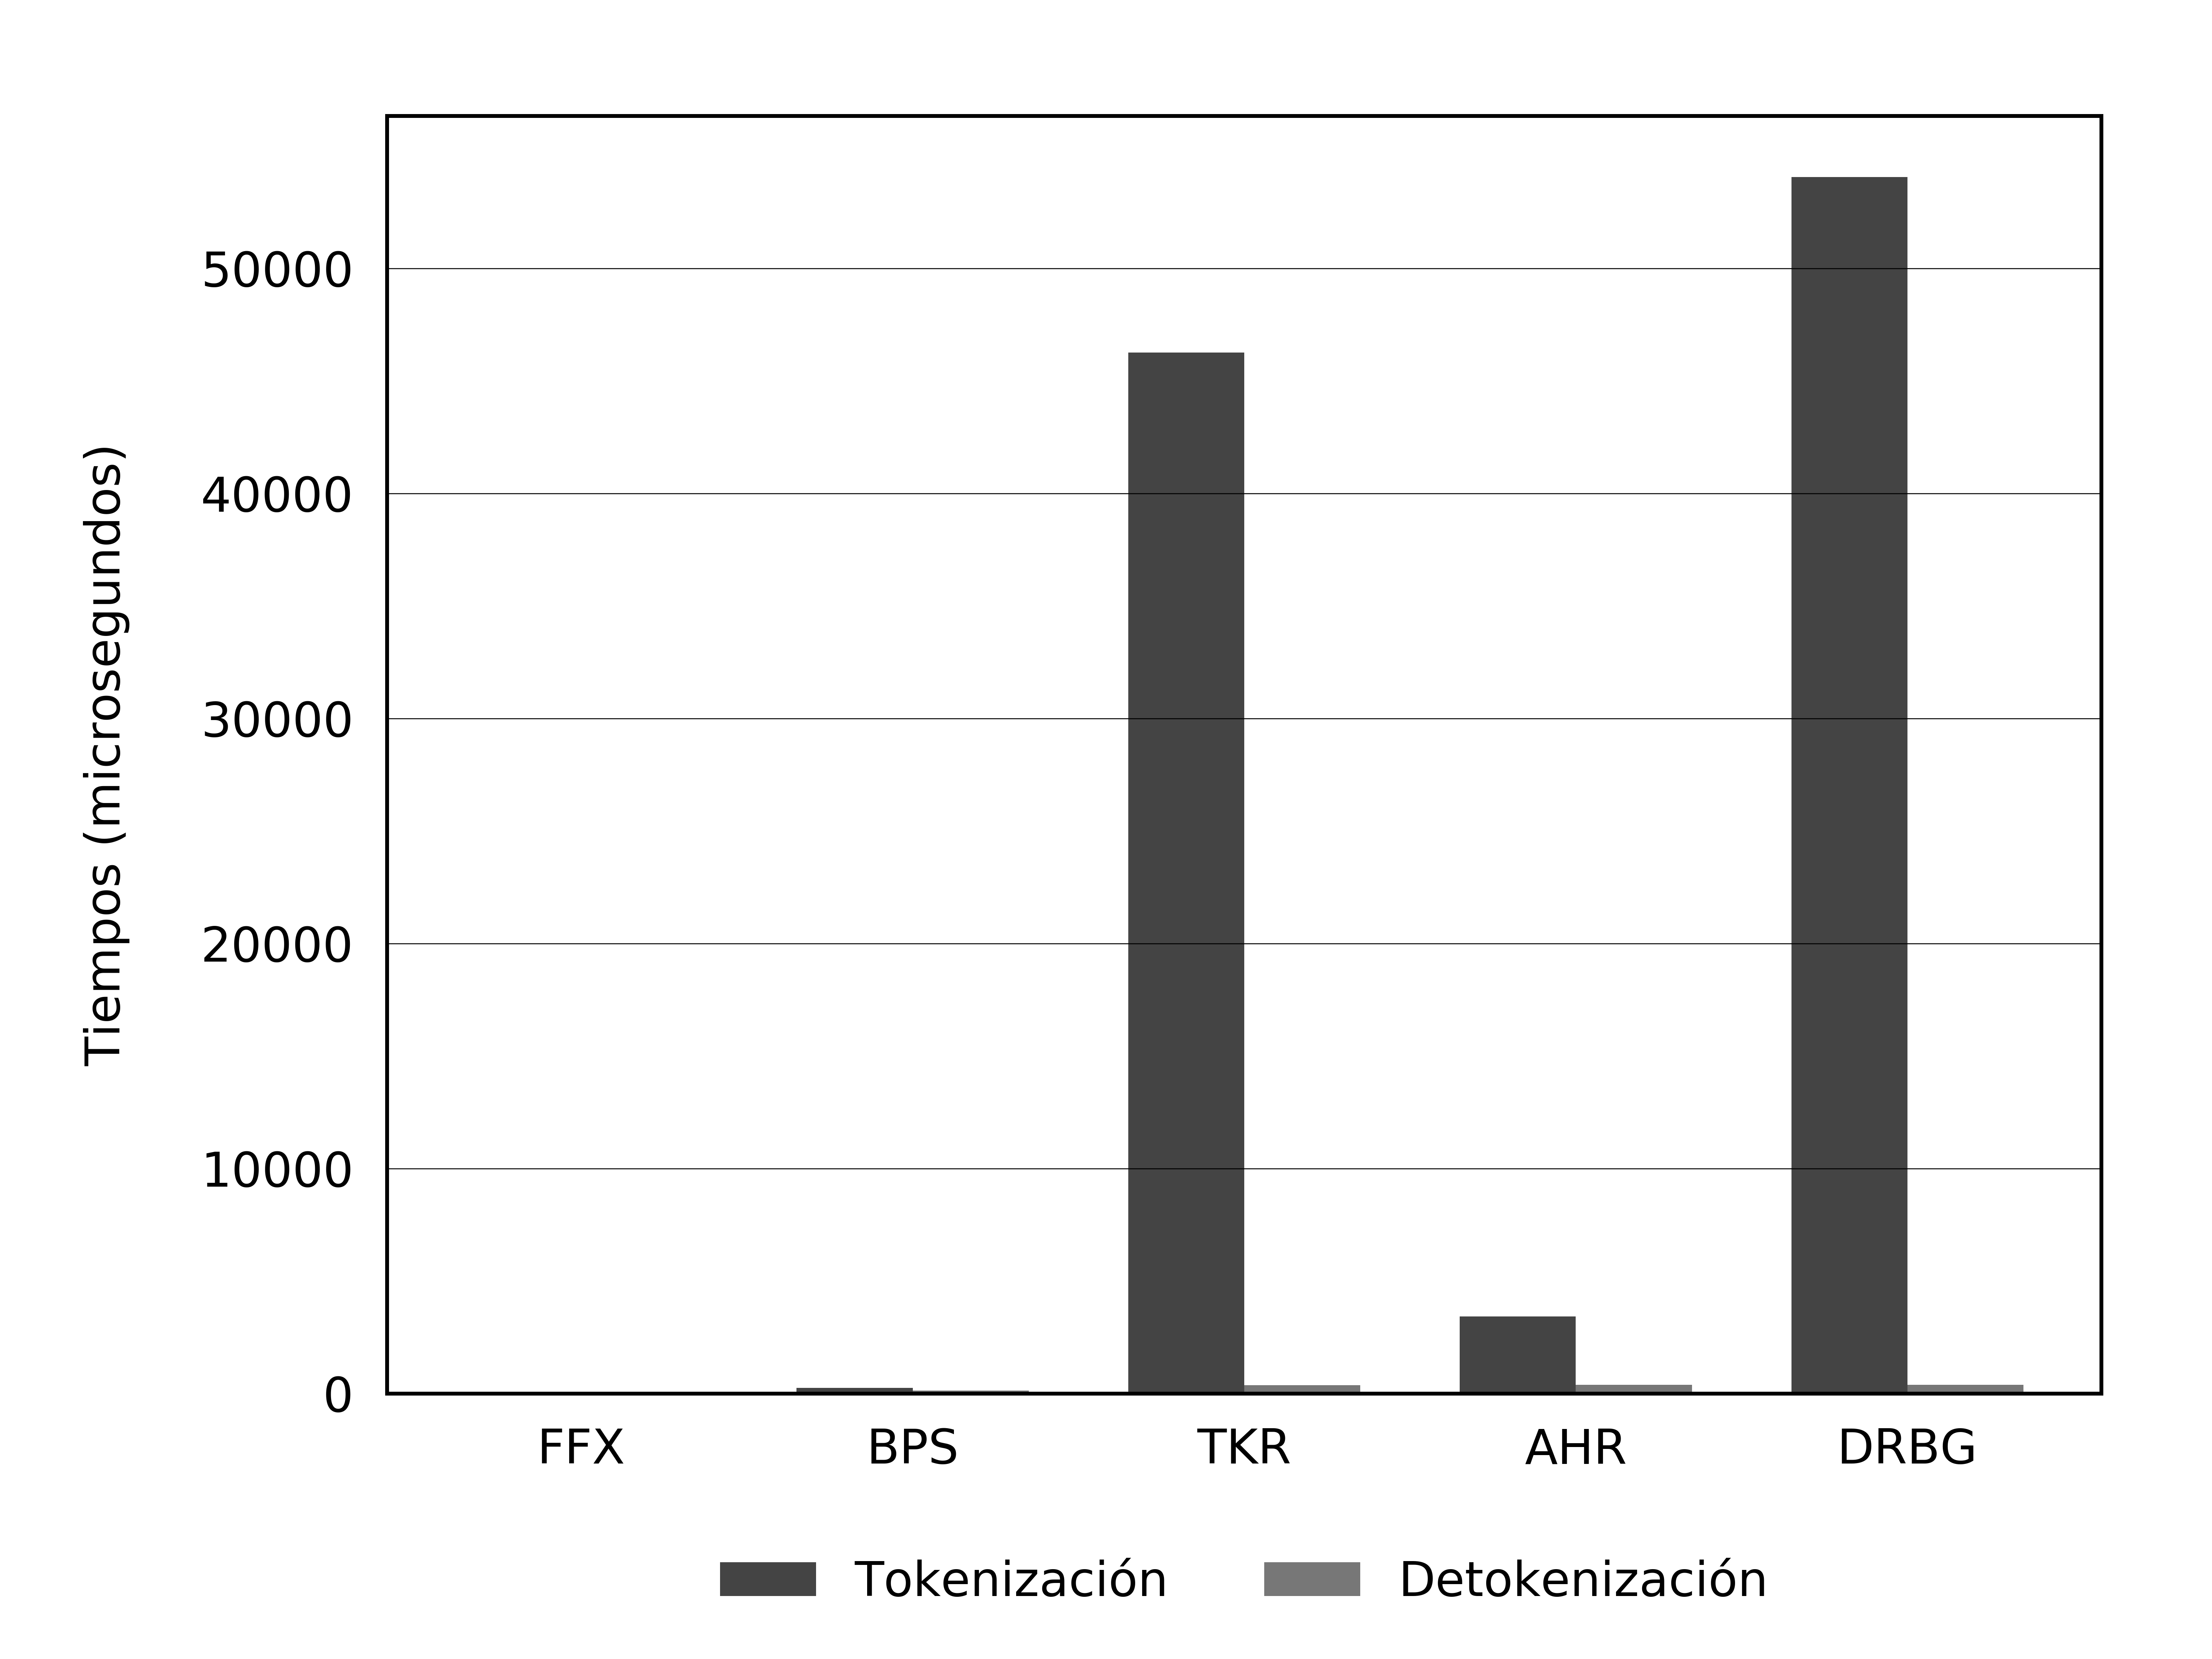
\includegraphics[width=1.0\linewidth]
      {../implementaciones/reportes/tiempos_unitarios.png}
    \caption{Comparación de tiempos de tokenización.}
    \label{figura:tiempos_tokenizacion}
  \end{center}
\end{figure}
